\begin{figure*}[t]
  \centering
  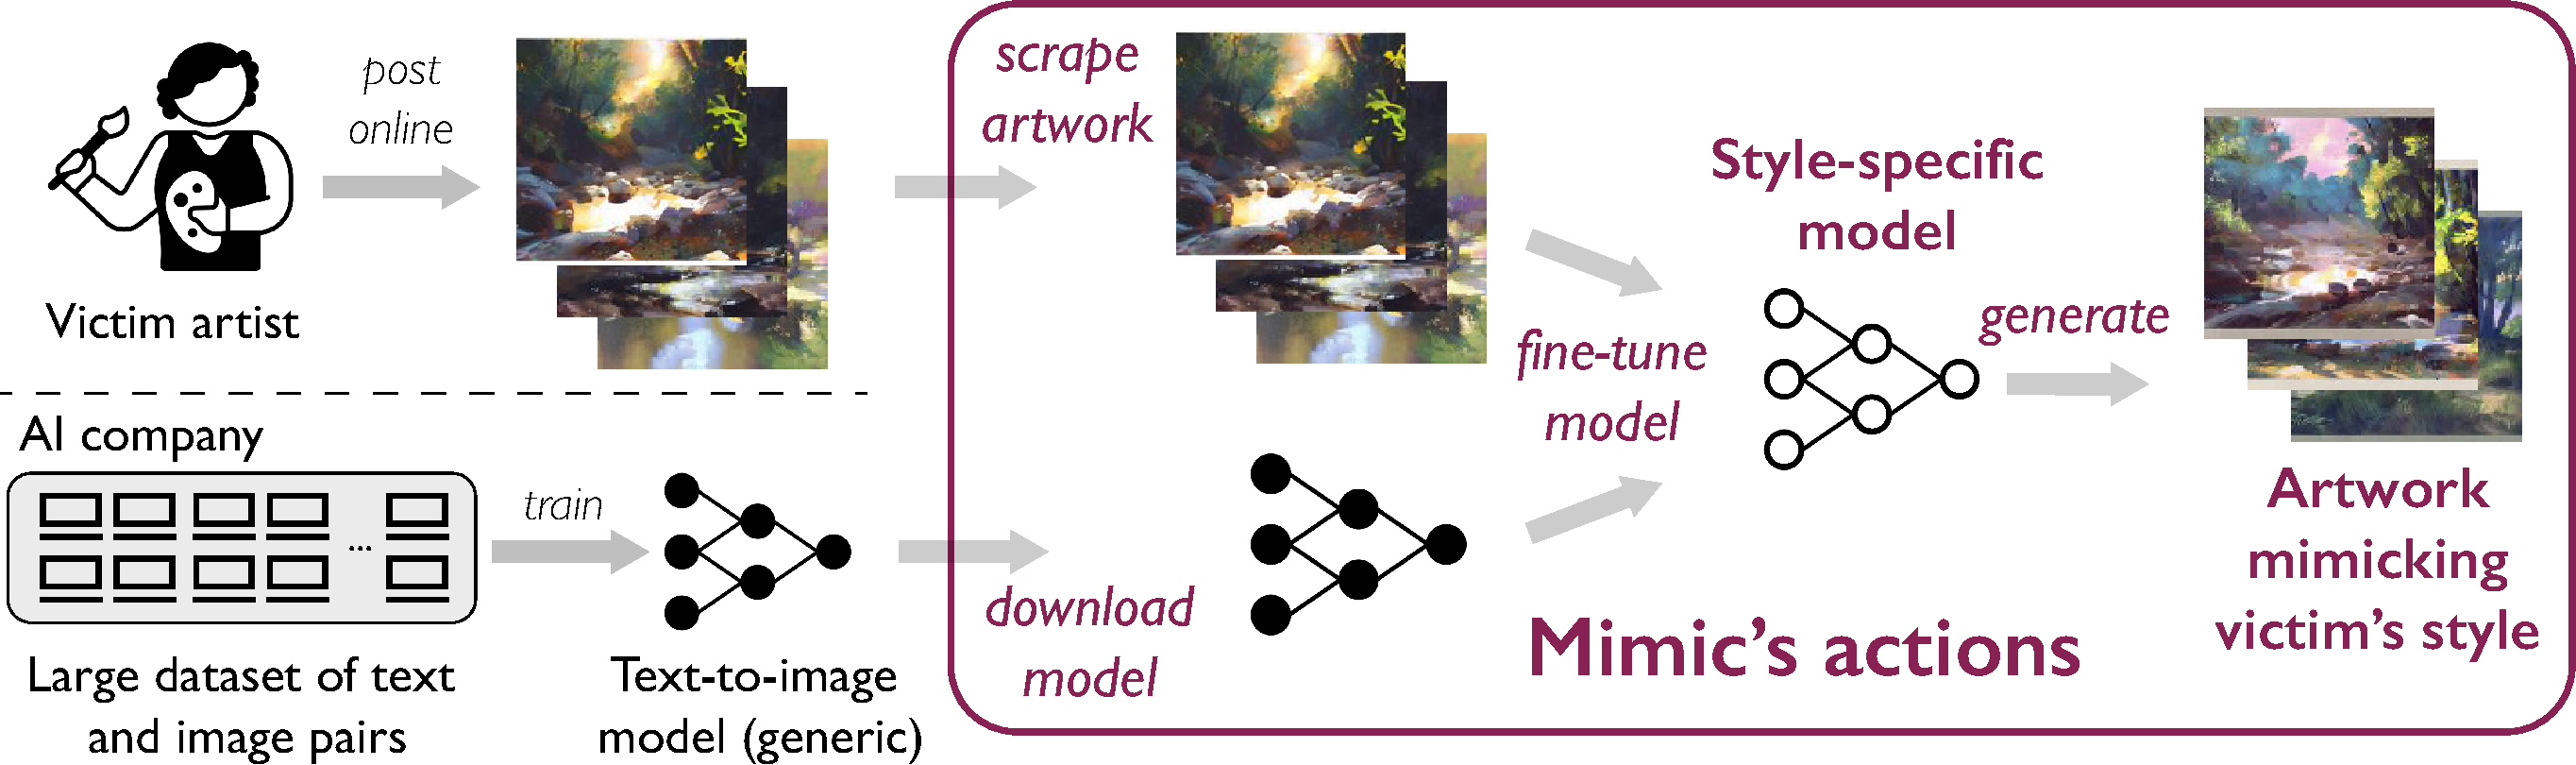
\includegraphics[width=0.85\linewidth]{plots/overview/attack-scenario-emily.pdf}
  \caption{High level overview of the mimicry attack scenario. The mimic scrapes copyrighted artwork from the victim artist and uses these to fine-tune a pre-trained, generic text-to-image model. \shawn{The generic model is trained and open-sourced by an AI company. }The mimic then uses the fine-tuned model to generate artwork in the style of the victim artist. }
  \label{fig:scenario}
\end{figure*}

\secspace
\section{Preliminaries}
\label{sec:cloak}

We propose \system{}, a tool that protects artists against AI
style mimicry. An artist uses \system{} to add small digital perturbations
(``cloak'') to images of their own art before sharing online
(Figure~\ref{fig:cloaking}). A text-to-image model that trains on cloaked
images of artwork will learn an incorrect representation of the artist's style in
feature space \ie the model's internal understanding of artistic styles. When
asked to generate art pieces in victim's style, the model will fail to mimic
the style of the victim, and instead output art pieces in a recognizably 
different style. 

Here, we first introduce the threat model, then discuss existing alternatives
to the AI style mimicry problem. We present the intuition behind \system{} and detailed
design in \S\ref{sec:design}.

\secspace
\subsection{Threat Model}

Here we state assumptions for both the artists protecting their own art
and the users training models to replicate their artistic style. We
refer to these AI art model trainers as ``mimics.''

% \todo{add on uncloaked and transferability, and countermeasures. }
\para{Artists.} Artists want to share and promote their artwork online
without allowing mimics to train models that replicate their art styles.
Sharing art online enables artists to sell their work and attract
commissioned work, fueling their livelihoods~(\S\ref{sec:artists}). Artists
protect themselves by adding imperceptible perturbations to their artwork
before sharing them as shown in Figure~\ref{fig:cloaking}. The goal of the
\system{} cloak is to disrupt the style mimicry process, while only
introducing minimal perturbation on images of the artwork.

We assume the artists have access to moderate computing resources (\eg a
laptop) and add perturbation to images of their artwork locally before
posting online. We also assume artists have access to some public feature
extractor (\eg open-source models such as Stable Diffusion). We begin with
assumption that artists use the same feature extractor as mimics (large
majority of mimics use the open-source Stable Diffusion model). We later
relax this assumption.

\para{Mimics. } The mimic's goal is to train a text-to-image model that
generates \emph{high-quality} art pieces of any subject in the \emph{victim's
  style}. A mimic could be a well-funded AI company, \eg Stability AI or
OpenAI, or an individual interested in the style of victim artist. We assume
the mimic has:

\vspace{-0.1cm}
\begin{packed_itemize}
\item access to the weights of generic text-to-image models well-trained on large datasets;
\item access to art pieces from the target artist;
\item significant computational power. 
\end{packed_itemize}

\vspace{-0.1cm}
We assume the attack scenario where the mimic 
fine-tunes its model on images of the artist's artwork (as shown in
Figure~\ref{fig:scenario}). This is stronger than the naive mimic attack
without fine tuning. 
Finally, we assume the mimic is aware of our
protection tool and can deploy adaptive countermeasures (\S\ref{sec:counter}).  

\secspace
\subsection{Potential Alternatives and Challenges}
\label{sec:challenge}

A number of related prior works target protection against invasive and
unauthorized facial recognition models. They proposed ``image cloaking'' as a
tool to prevent a user's images from being used to train a facial recognition
model of
them~\cite{shan2020fawkes,cherepanova2021lowkey,chandrasekaran2020face,evtimov2020foggysight,wenger2021sok}. They
share a similar high level approach, by using optimized perturbations that
cause cloaked images to have drastically different feature representations
from original user images. % A face recognition model trained on cloaked images
% will associate an incorrect feature representation with an user's identity
% and thus will fail to recognize the user at inference time.
It is possible to
adapt existing cloaking-based systems to protect artists against AI style
mimicry. Protection system would compute a cloak on each artwork in order
to perturb its feature space representation to be different from its
unperturbed representation. This can succeed if the cloak significantly shifts
the artwork's feature representation, making resulting models generate
dramatically different artwork.

We found that in practice, however, existing solutions are unable to
introduce large-enough feature space shifts to achieve the desired
protection. This is due to the properties of feature spaces in text-to-image
models. Face recognition models {\em classify identities}, so their feature
spaces mainly represent identity-related information. On the other hand,
text-to-image models {\em reconstruct original images from extracted
  features}, so their feature spaces retain more information about the
original image (objects, locations, color, style, etc.). Thus, producing the
same shift in feature representation in a text-to-image model is much harder
(requires more perturbation budget) than in a classification model. This
observation is validated by prior work showing that adversarial perturbations
are much less effective at attacking generative
models~\cite{kos2018adversarial,gondim2018adversarial,tabacof2016adversarial}. Specifically,
\cite{kos2018adversarial,tabacof2016adversarial} found that adversarial
attack methods that are effective at attacking classifiers are significantly
less effective at attacking autoencoders. We empirically confirm that
existing cloaking methods cannot prevent AI mimicry (\S\ref{app:prior-work}
in Appendix). We show that Fawkes~\cite{shan2020fawkes} and
LowKey~\cite{cherepanova2021lowkey} perform poorly in this setting, even when
artists add highly visible cloaks to their artwork.

For generative models, concurrent work~\cite{madry-defense}
proposes PhotoGuard, a method to cloak images to prevent
unauthorized image edits (inpainting) on cloaked images. Similar to existing
cloaking systems, PhotoGuard tries to indiscriminately minimize all
information contained in an image (\ie the norm of the feature vector) to
prevent models from editing the image. Thus, it is also not effective at
mimicry prevention.  


\para{Design Challenges. } The main reason that existing cloaking methods
fail to prevent AI mimicry is because they indiscriminately shift all
features in an image, wasting the cloak perturbation budget on shifting
unnecessary features (\eg object shape, location, etc.). Protecting artist's
style requires only {\em shifting features related to the artistic style of
  victim}. This can be achieved if a text-to-image model learns to draw objects
similar to those drawn by the victim artist {\em as long as the model cannot
  mimic the artist's unique style}. Thus, optimal protection from mimicry requires
concentrating the cloak on style-specific features.  

Unfortunately, identifying and separating out these style-specific features
is difficult. Even assuming the existence of interpretability methods that
perfectly explain the feature space of a text-to-image model, there is no
clear way to mathematically define and calculate ``artistic styles.'' In all
likelihood, any definition would change across different styles. For example,
``impressionist'' likely correlates more strongly with color features,
whereas ``cubism'' correlates with shape features. Even across multiple
art pieces in the same style, the style may manifest differently.  
